% Transmission Electron Microscope System
% Author: Eric Jensen
\documentclass[border=10pt,tikz]{standalone}
\usepackage{tikz}
\usetikzlibrary{calc, decorations.pathmorphing, fadings, shadings}

\begin{document}
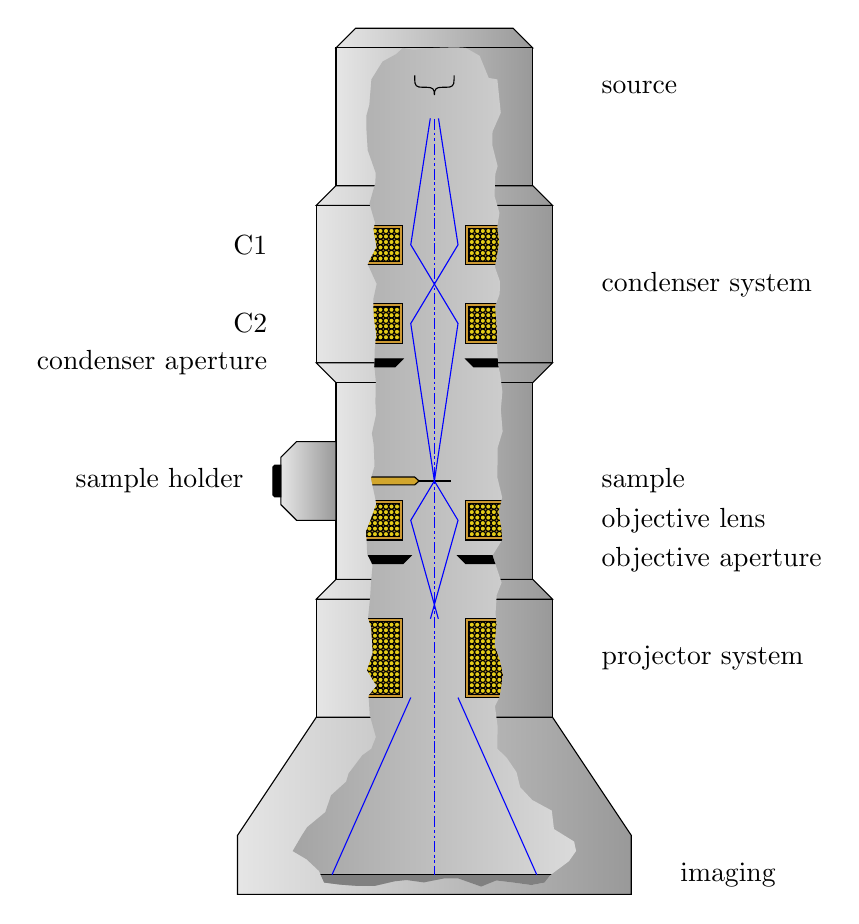
\begin{tikzpicture}
	\draw[gray,fill=gray,path fading=south] (0,0) rectangle +(0.3,-0.3);% <- MAGIC
		% (if this is not present none of the shadings work)

	%top
	\shade[left color=black!10!white,right color=black!40!white] (-1,0.75)
		-- ++(2,0) -- ++(0.25,-0.25) -- ++(-2.5,0) -- cycle;
	\draw (-1,0.75) -- ++(2,0) -- ++(0.25,-0.25) -- ++(-2.5,0) -- cycle;

	%source
	\shade[left color=black!10!white,right color=black!40!white] (1.25,0.5)
		-- ++(0,-1.75) -- ++(-2.5,0) -- ++(0,1.75) -- cycle;
	\draw (1.25,0.5) -- ++(0,-1.75) -- ++(-2.5,0) -- ++(0,1.75) -- cycle;

	%top condenser system
	\shade[left color=black!10!white,right color=black!40!white] (1.25,-1.25)
		-- ++(0.25,-0.25) -- ++(-3,0) -- ++(0.25,0.25) -- cycle;
	\draw (1.25,-1.25) -- ++(0.25,-0.25) -- ++(-3,0) -- ++(0.25,0.25) -- cycle;

	%condenser system
	\shade[left color=black!10!white,right color=black!40!white] (1.5,-1.5)
		-- ++(0,-2) -- ++(-3,0) -- ++(0,2) -- cycle;
	\draw (1.5,-1.5) -- ++(0,-2) -- ++(-3,0) -- ++(0,2) -- cycle;

	%condenser bottom
	\shade[left color=black!10!white,right color=black!40!white] (1.5,-3.5)
		-- ++(-0.25,-0.25) -- ++(-2.5,0) -- ++(-0.25,0.25) -- cycle;
	\draw (1.5,-3.5) -- ++(-0.25,-0.25) -- ++(-2.5,0) -- ++(-0.25,0.25) -- cycle;

	%specimen and objective
	\shade[left color=black!10!white,right color=black!40!white] (1.25,-3.75)
		-- ++(0,-2.5) -- ++(-2.5,0) -- ++(0,2.5) -- cycle;
	\draw (1.25,-3.75) -- ++(0,-2.5) -- ++(-2.5,0) -- ++(0,2.5) -- cycle;

	%projector system top
	\shade[left color=black!10!white,right color=black!40!white] (1.25,-6.25)
		-- ++(0.25,-0.25) -- ++(-3,0) -- ++(0.25,0.25) -- cycle;
	\draw (1.25,-6.25) -- ++(0.25,-0.25) -- ++(-3,0) -- ++(0.25,0.25) -- cycle;

	%projector system
	\shade[left color=black!10!white,right color=black!40!white] (1.5,-6.5)
		-- ++(0,-1.5) -- ++(-3,0) -- ++(0,1.5) -- cycle;
	\draw (1.5,-6.5) -- ++(0,-1.5) -- ++(-3,0) -- ++(0,1.5) -- cycle;

	%image
	\shade[left color=black!10!white,right color=black!40!white] (1.5,-8)
		-- ++(1,-1.5) -- ++(0,-0.75) -- ++(-5,0) -- ++(0,0.75) -- ++(1,1.5) -- cycle;
	\draw (1.5,-8) -- ++(1,-1.5) -- ++(0,-0.75) -- ++(-5,0) -- ++(0,0.75)
		-- ++(1,1.5) -- cycle;

	%sample entrance
	\shade[left color=black!10!white,right color=black!40!white] (-1.25,-4.5)
		-- ++(-0.5,0) -- ++(-0.2,-0.2) -- ++(0,-0.6) -- ++(0.2,-0.2)
		-- ++(0.5,0) -- cycle;
	\draw (-1.25,-4.5) -- ++(-0.5,0) -- ++(-0.2,-0.2) -- ++(0,-0.6)
		-- ++(0.2,-0.2)  -- ++(0.5,0) -- cycle;

	%sample holder
	\draw[fill=black] (-1.95,-4.8) -- ++(-0.08,0) -- ++(-0.02,-0.02)
		-- ++(0,-0.36) -- ++(0.02,-0.02) -- ++(0.08,0) -- cycle;

	%inside
	\begin{scope}
		\path[clip,decoration={random steps, segment length=6pt, amplitude=2pt},
			decorate] (0,0.5) -- ++(0.4,0) -- ++(0.4,-0.4) -- ++(0,-8.5)
			-- ++(1,-1.3) -- ++(-0.4,-0.4) -- ++(-2.8,0) -- ++(-0.4,0.4)
			-- ++(1,1.3) -- ++(0,8.5) -- ++(0.4,0.4) -- cycle;
		\shade[left color=black!40!white,right color=black!10!white] (-1,0.75)
			-- ++(2,0) -- ++(0.25,-0.25) -- ++(0,-1.75) -- ++(0.25,-0.25) -- ++(0,-2)
			-- ++(-0.25,-0.25) -- ++(0,-2.5) -- ++(0.25,-0.25) -- ++(0,-1.5)
			-- ++(1,-1.5) -- ++(0,-0.75) -- ++(-5,0) -- ++(0,0.75) -- ++(1,1.5)
			-- ++ (0,1.5) -- ++(0.25,0.25) -- ++(0,2.5) -- ++(-0.25,0.25) -- ++(0,2)
			-- ++(0.25,0.25) -- ++(0,1.75) -- cycle;
 
 	%source
	\draw (-0.25,0.15) -- ++(0,-0.05) .. controls +(0,-0.08) and +(-0.08,0)
		.. ++(0.1,-0.1) -- ++(0.05,0) .. controls +(0.08,0) and +(0,0.08)
		.. ++(0.1,-0.1) .. controls +(0,0.08) and +(-0.08,0) .. ++(0.1,0.1) --
		++(0.05,0) .. controls +(0.08,0) and +(0,-0.08) .. ++(0.1,0.1) -- ++(0,0.05);

	%C1
	\draw[fill=brown!80!yellow] (-0.4,-1.75) -- ++(-0.5,0) -- ++(0,-0.5)
		-- ++(0.5,0) -- cycle;
	\draw (-0.4,-1.75) ++(-0.04,-0.04) -- ++(-0.42,0) -- ++(0,-0.42)
		-- ++(0.42,0) -- cycle;
	\begin{scope}
		\path[clip,draw] (-0.4,-1.75) ++(-0.04,-0.04) -- ++(-0.42,0)
			-- ++(0,-0.42) -- ++(0.42,0) -- cycle;
		\foreach \j in {-0.07,-0.14,...,-0.42}
			\foreach \i in {-0.07,-0.14,...,-0.42} {
				\draw[fill=brown!40!yellow] (-0.4,-1.75) ++(-0.04,-0.04)
					++(0.035,0.035) ++(\i,\j) circle (0.035);
			}
	\end{scope}
	\draw[fill=brown!80!yellow] (0.9,-1.75) -- ++(-0.5,0) -- ++(0,-0.5)
		-- ++(0.5,0) -- cycle;
	\draw (0.9,-1.75) ++(-0.04,-0.04) -- ++(-0.42,0) -- ++(0,-0.42)
		-- ++(0.42,0) -- cycle;
	\begin{scope}
		\path[clip,draw] (0.9,-1.75) ++(-0.04,-0.04) -- ++(-0.42,0)
			-- ++(0,-0.42) -- ++(0.42,0) -- cycle;
		\foreach \j in {-0.07,-0.14,...,-0.42}
			\foreach \i in {-0.07,-0.14,...,-0.42} {
				\draw[fill=brown!40!yellow] (0.9,-1.75) ++(-0.04,-0.04)
					++(0.035,0.035) ++(\i,\j) circle (0.035);
			}
	\end{scope}

	%C2
	\draw[fill=brown!80!yellow] (-0.4,-2.75) -- ++(-0.5,0) -- ++(0,-0.5)
		-- ++(0.5,0) -- cycle;
	\draw (-0.4,-2.75) ++(-0.04,-0.04) -- ++(-0.42,0) -- ++(0,-0.42)
		-- ++(0.42,0) -- cycle;
	\begin{scope}
		\path[clip,draw] (-0.4,-2.75) ++(-0.04,-0.04) -- ++(-0.42,0)
			-- ++(0,-0.42) -- ++(0.42,0) -- cycle;
		\foreach \j in {-0.07,-0.14,...,-0.42}
			\foreach \i in {-0.07,-0.14,...,-0.42} {
				\draw[fill=brown!40!yellow] (-0.4,-2.75) ++(-0.04,-0.04)
					++(0.035,0.035) ++(\i,\j) circle (0.035);
			}
	\end{scope}
	\draw[fill=brown!80!yellow] (0.9,-2.75) -- ++(-0.5,0) -- ++(0,-0.5)
		-- ++(0.5,0) -- cycle;
	\draw (0.9,-2.75) ++(-0.04,-0.04) -- ++(-0.42,0) -- ++(0,-0.42)
		-- ++(0.42,0) -- cycle;
	\begin{scope}
		\path[clip,draw] (0.9,-2.75) ++(-0.04,-0.04) -- ++(-0.42,0)
			-- ++(0,-0.42) -- ++(0.42,0) -- cycle;
		\foreach \j in {-0.07,-0.14,...,-0.42}
			\foreach \i in {-0.07,-0.14,...,-0.42} {
				\draw[fill=brown!40!yellow] (0.9,-2.75) ++(-0.04,-0.04)
					++(0.035,0.035) ++(\i,\j) circle (0.035);
			}
	\end{scope}

	%condenser aperture
	\draw[fill=black] (-1,-3.45) -- ++(0.6,0) -- ++(-0.1,-0.1)
		-- ++(-0.5,0) -- cycle;
	\draw[fill=black] (1,-3.45) -- ++(-0.6,0) -- ++(0.1,-0.1)
		-- ++(0.5,0) -- cycle;

	%specimen
	\draw[fill=brown!70!yellow] (-1,-4.95) -- ++(0.75,0) -- ++(0.05,-0.045)
		-- ++(0,-0.01) -- ++(-0.05,-0.045) -- ++(-0.75,0) -- cycle;
	\draw[fill=black] (-0.2,-4.995) -- ++(0.4,0) -- ++(0,-0.01)
		-- ++(-0.4,0) -- cycle;
		
	%objective
	\draw[fill=brown!80!yellow] (-0.4,-5.25) -- ++(-0.5,0) -- ++(0,-0.5)
		-- ++(0.5,0) -- cycle;
	\draw (-0.4,-5.25) ++(-0.04,-0.04) -- ++(-0.42,0) -- ++(0,-0.42)
		-- ++(0.42,0) -- cycle;
	\begin{scope}
		\path[clip,draw] (-0.4,-5.25) ++(-0.04,-0.04) -- ++(-0.42,0)
			-- ++(0,-0.42) -- ++(0.42,0) -- cycle;
		\foreach \j in {-0.07,-0.14,...,-0.42}
			\foreach \i in {-0.07,-0.14,...,-0.42} {
				\draw[fill=brown!40!yellow] (-0.4,-5.25) ++(-0.04,-0.04)
					++(0.035,0.035) ++(\i,\j) circle (0.035);
			}
	\end{scope}
	\draw[fill=brown!80!yellow] (0.9,-5.25) -- ++(-0.5,0) -- ++(0,-0.5)
		-- ++(0.5,0) -- cycle;
	\draw (0.9,-5.25) ++(-0.04,-0.04) -- ++(-0.42,0) -- ++(0,-0.42)
		-- ++(0.42,0) -- cycle;
	\begin{scope}
		\path[clip,draw] (0.9,-5.25) ++(-0.04,-0.04) -- ++(-0.42,0)
			-- ++(0,-0.42) -- ++(0.42,0) -- cycle;
		\foreach \j in {-0.07,-0.14,...,-0.42}
			\foreach \i in {-0.07,-0.14,...,-0.42} {
				\draw[fill=brown!40!yellow] (0.9,-5.25) ++(-0.04,-0.04)
					++(0.035,0.035) ++(\i,\j) circle (0.035);
			}
	\end{scope}
		
	%objective aperture
	\draw[fill=black] (-1,-5.95) -- ++(0.7,0) -- ++(-0.1,-0.1)
		-- ++(-0.6,0) -- cycle;
	\draw[fill=black] (1,-5.95) -- ++(-0.7,0) -- ++(0.1,-0.1)
		-- ++(0.6,0) -- cycle;
		
		

	%projector system
	\draw[fill=brown!80!yellow] (-0.4,-6.75) -- ++(-0.5,0)
		-- ++(0,-1) -- ++(0.5,0) -- cycle;
	\draw (-0.4,-6.75) ++(-0.04,-0.04) -- ++(-0.42,0) -- ++(0,-0.92)
		-- ++(0.42,0) -- cycle;
	\begin{scope}
		\path[clip,draw] (-0.4,-6.75) ++(-0.04,-0.04) -- ++(-0.42,0)
			-- ++(0,-0.92) -- ++(0.42,0) -- cycle;
		\foreach \j in {-0.07,-0.14,...,-0.92}
			\foreach \i in {-0.07,-0.14,...,-0.42} {
				\draw[fill=brown!40!yellow] (-0.4,-6.75) ++(-0.04,-0.04)
					++(0.035,0.035) ++(\i,\j) circle (0.035);
			}
	\end{scope}
	\draw[fill=brown!80!yellow] (0.9,-6.75) -- ++(-0.5,0) -- ++(0,-1)
		-- ++(0.5,0) -- cycle;
	\draw (0.9,-6.75) ++(-0.04,-0.04) -- ++(-0.42,0) -- ++(0,-0.92)
		-- ++(0.42,0) -- cycle;
	\begin{scope}
		\path[clip,draw] (0.9,-6.75) ++(-0.04,-0.04) -- ++(-0.42,0)
			-- ++(0,-0.92) -- ++(0.42,0) -- cycle;
		\foreach \j in {-0.07,-0.14,...,-0.92}
			\foreach \i in {-0.07,-0.14,...,-0.42} {
				\draw[fill=brown!40!yellow] (0.9,-6.75) ++(-0.04,-0.04)
					++(0.035,0.035) ++(\i,\j) circle (0.035);
			}
	\end{scope}

	%image
	\draw[fill=gray] (2,-10) -- ++(0,-0.2) -- ++(-4,0) -- ++(0,0.2) -- cycle;
		
	%beam
	\draw[blue] (0,-0.1) ++(260:0.3) -- (-0.3,-2) -- ++(0.6,-1) -- ++(-0.3,-2)
		-- ++(-0.3,-0.5) -- ++(0.35,-1.25);
	\draw[blue] (0,-0.1) ++(280:0.3) -- (0.3,-2) -- ++(-0.6,-1) -- ++(0.3,-2)
		-- ++(0.3,-0.5) -- ++(-0.35,-1.25);
	\draw[blue] (-0.3,-7.75) -- ++(-1,-2.25);
	\draw[blue] (0.3,-7.75) -- ++(1,-2.25);
	\draw[blue,dash pattern=on 4pt off 1pt on 1pt off 1pt on 1pt off 1pt]
		(0,-0.4) -- (0,-10);

	\end{scope}

	%labels
	\draw (2,0) node[right] {source};
	\draw (-2,-2) node[left] {C1};
	\draw (-2,-3) node[left] {C2};
	\draw (-2,-3.5) node[left] {condenser aperture};
	\draw (2,-2.5) node[right] {condenser system};
	\draw (2,-5) node[right] {sample};
	\draw (-2.3,-5) node[left] {sample holder};
	\draw (2,-5.5) node[right] {objective lens};
	\draw (2,-6) node[right] {objective aperture};
	\draw (2,-7.25) node[right] {projector system};
	\draw (3,-10) node[right] {imaging};

	\end{tikzpicture}
\end{document}